\documentclass[12pt,a4j,titlepage]{ltjsarticle}
\usepackage{semi}
\setcounter{tocdepth}{3}


\begin{document}
\begin{titlepage}
  \centering
    \vspace*{40truept}
    {\LARGE 2023年度 卒業論文}
    
    \vspace*{75truept}
    
    {\Huge カラーユニバーサルデザイン}
\vspace*{18truept}

    {\Huge (CUD)の学習支援ツールの開発}%論文タイトル

    \vspace{85truept}
    
    {\LARGE 指導教員 須田 宇宙 准教授}
    
    \vspace{60truept}
    
    {\LARGE 千葉工業大学 情報ネットワーク学科}
    
    \vspace{15truept}
    
    {\LARGE 須田研究室}
    
    \vspace{70truept}
    
    {\LARGE 2032116 氏名 永溝 柊介 } % 氏名は消さない 学生番号 氏名 名前

    \vspace{70truept}
    
  \begin{flushright}

    \LARGE {提出日 2024年1月19日}
  
  \end{flushright}
\end{titlepage}
\date{}

\tableofcontents
\newpage
\listoftables
\newpage
\listoffigures
\newpage

%1章
\section{緒言}

%背景1
遺伝子の異常により通常と色の見え方が異なる色覚を持つ色覚異常者は,男性で5%,女性で0.2%存在する\cite{okabe}.
色覚異常には,主に赤を感じづらいP型色覚,緑を感じづらいD型色覚,青を感じづらいT型色覚がある.
色覚の多様性に配慮し,より多くの人に伝わりやすいデザインとしてカラーユニバーサルデザイン(CUD)がある.

%背景2
学生や社会人になると,ゼミや業務等で資料を作成する機会が増加する.
そのため,CUDの講習では資料作成を実践し評価する機会が設けられている.
しかし,講習を受けた学生の20%がCUDに配慮していない資料を作成した\cite{sugamiya}.
先行研究では,講習内容を即座に理解することが困難なためと考察されている.
そのため,CUDに配慮した工夫を一つ一つ実践する機会が必要だと考える.

%問題点
学習者は別色覚での見え方を確認することでCUDをより理解できると考えられるが,現状では別媒体のシミュレータを使う必要がある.
また,評価者にとって学習者の作成物のCUD適合度を即座に判断することが難しく,評価や改善案を即座に提示することは困難である.
そのため,学習の際は,別色覚での見え方を即座に確認でき,自動で評価・改善案の提示を行う環境が望ましい.

%目的
そこで本研究では,これらの環境を持ち,CUDに配慮した工夫を項目ごとに実践できる学習ツールの開発を行う.
そして,開発した学習ツールを学習者が利用することでCUDに配慮した資料を作成できるか検証することを目的とする.


\clearpage

%2章
\section{色覚異常とカラーユニバーサルデザイン(CUD)について}
本章では,色覚異常とCUDについて説明する.

\subsection{色覚異常について}
人間の目には,赤,緑,青の3種類をそれぞれ感じる機能を持つ錐体があり,その錐体によって色を識別している.
この錐体の一部が十分に機能しないために,通常とは色の見え方が異なる色覚となる場合がある.
このような色覚を持つ色覚異常者は,日本人の場合,男性で5%,女性で0.2%存在する.

色覚異常者は,主にどの色を感じづらい色覚かによって区別される.
主に赤を感じづらい色覚であるP型色覚は,全体の約25%を占める.
主に緑を感じづらい色覚であるD型色覚は,全体の約75%を占める.
主に青を感じづらい色覚であるT型色覚は,全体の約0.02%を占める.

\subsection{色覚異常の見え方とCUDについて}
図\ref{fig:pcolor_mae}は,同じグラフに対しての色覚による見え方の違いを表している.
左は通常の色覚での見え方,右はP型色覚での見え方を表している.
線1は緑色,線2は赤色であり,通常の色覚では区別がつきやすい.
しかし,P型色覚ではどちらも茶色に近い色に見えるため区別がつきづらい.
このように,通常の色覚者には伝わりやすい情報であっても,色覚異常者には伝わりづらくなっている場合がある.

\begin{figure}[h]
\begin{center}
 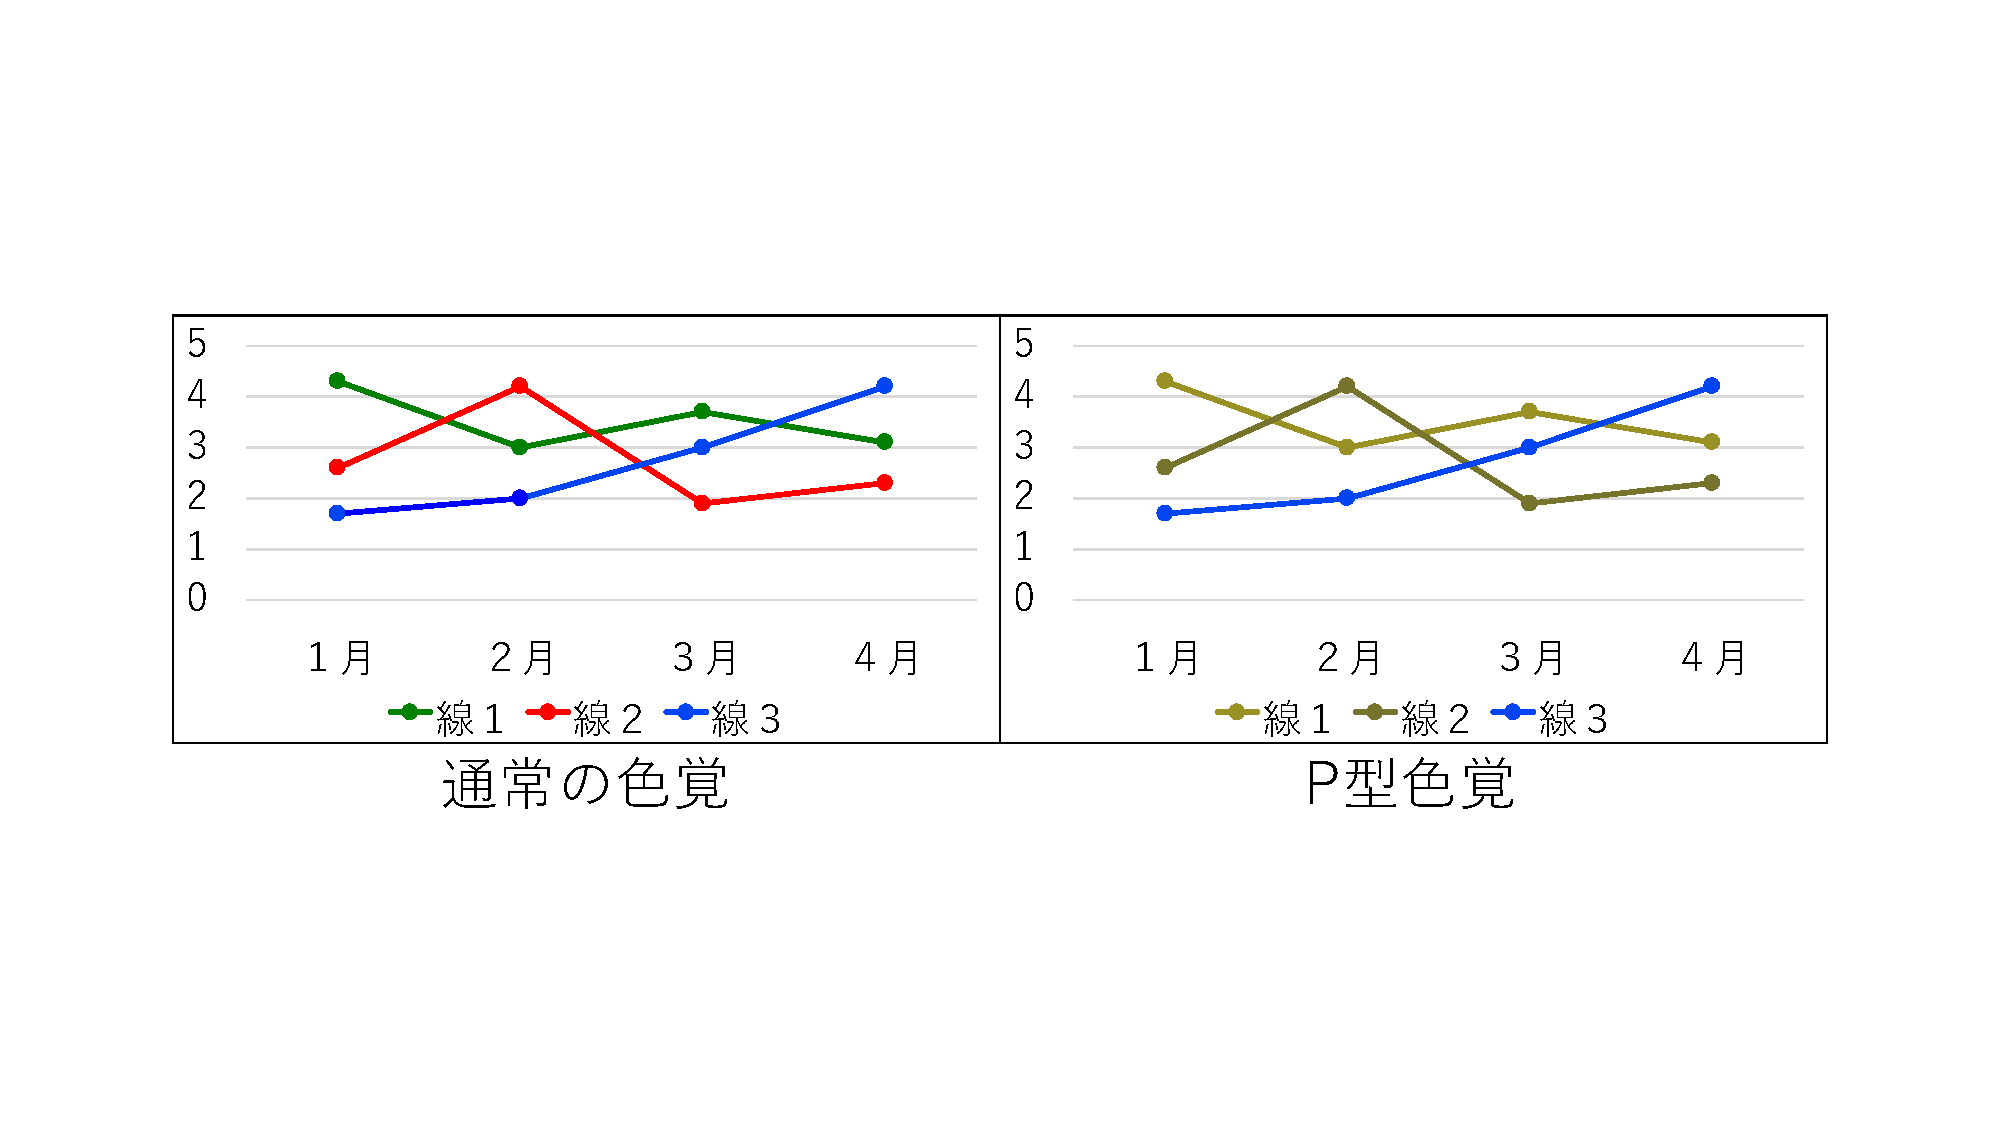
\includegraphics[clip,width=160mm,height=48mm]{images/pcolor_mae.pdf}
\end{center}
 \caption{P型色覚者の見え方}
 \label{fig:pcolor_mae}
\end{figure}

\clearpage

色覚の多様性に配慮し,より多くの人に伝わりやすい配色やデザインとして,CUDがある.
図\ref{fig:pcolor_ato}は,図\ref{fig:pcolor_ato}のグラフをCUDに配慮し,改善した例である.
図\ref{fig:pcolor_mae}と同様,左は通常の色覚での見え方,右はP型色覚での見え方を表している.
改善後のグラフでは,線2を橙色にし,点線にすることで区別がつきやすくした.
このように,色覚異常者にも正確に伝えるためには,CUDに配慮する必要がある.

\begin{figure}[h]
\begin{center}
 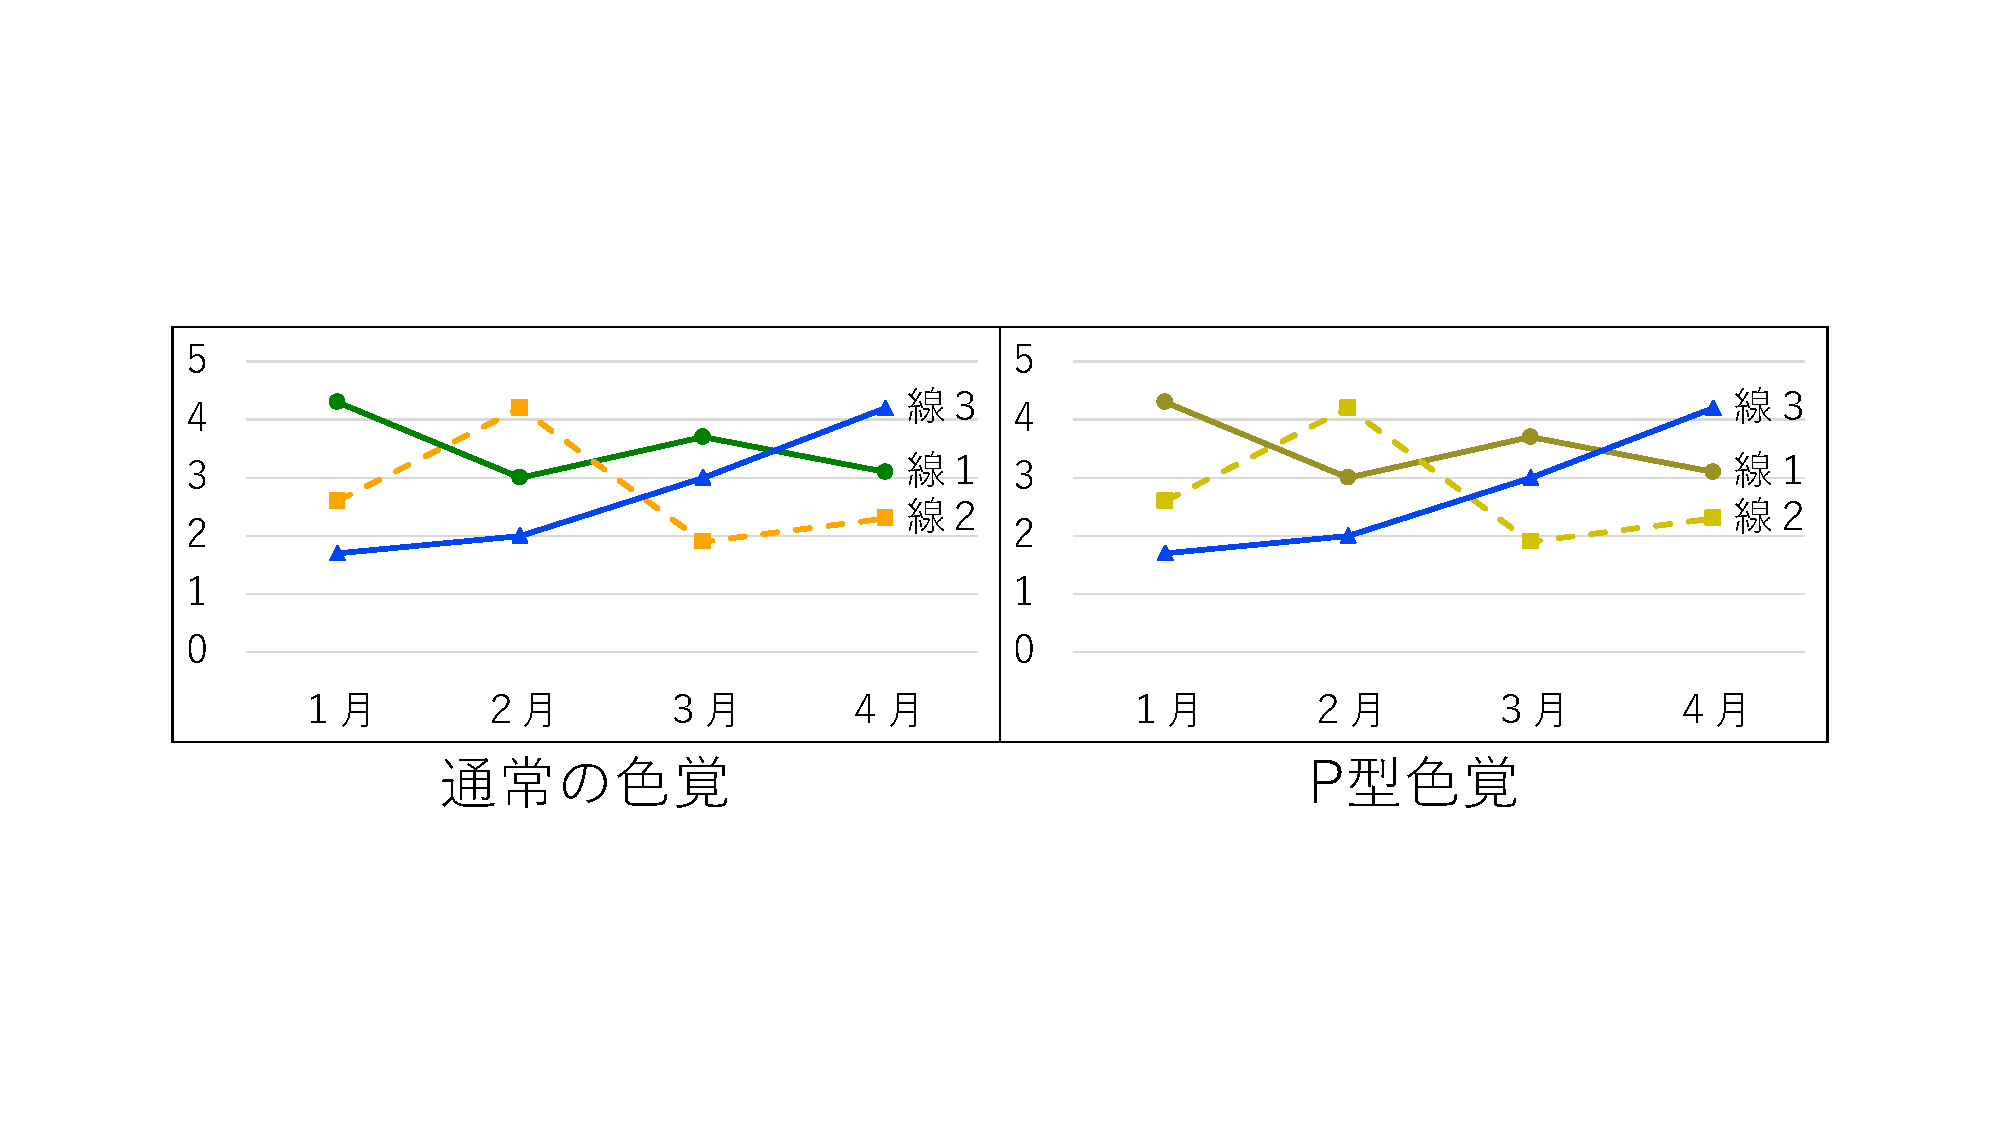
\includegraphics[clip,width=159mm,height=47mm]{images/pcolor_ato.pdf}
\end{center}
 \caption{改善後のグラフの見え方}
 \label{fig:pcolor_ato}
\end{figure}

\subsection{CUDの普及に向けた活動}
CUDの普及に向けた活動として,東京都は「カラーユニバーサルデザインガイドライン」を作成している\cite{tokyo}.
また,大阪府は「色覚障がいのある人に配慮した色使いのガイドライン」を作成している\cite{osaka}.
これらのように,一部の自治体がCUDの認知度を高めることを目的とし,CUDのガイドラインを作成している.

また,一部の大学,専門学校や会社では,講義や研修等を通してCUDに関する講習を行っている.




\clearpage

%3章
\section{CUD教育について}
本章では,CUD教育の内容と現状の課題について説明する.

\subsection{概要}
一般的に,色覚異常に関する講習では,主に色覚異常の見え方や色覚異常者にも伝わりやすいデザインであるCUDについての説明を行う.
CUD教育では,学習者が色覚異常に関する知識を得るだけでなく,資料等を作成する際にCUDに配慮した工夫を取り入れることができるようになることが求められる.
そのため,講義形式での説明に加え,学習者にCUDに配慮したデザインを体験してもらう場面が存在する.

大阪医療福祉専門学校でのCUDに関する授業では,色選びの体験ワークを行った\cite{jcolor}.
まず,学習者にゴミ分別に関する図の配色を考えさせた.
そして,色覚異常者の見え方を体験できるフィルター式眼鏡を掛けて,選択した色が色覚異常者でも区別できる配色となっているか確認させた.
このように,実際にCUDに配慮した図の作成を体験させる授業が行われた.

また,東京女子大学での講義では,色覚異常に関する説明の後にCUDに配慮した資料作成を実践する機会を設けていた\cite{sugamiya}.
この講義では,まず,東京都が作成したガイドライン等を参考に,色覚異常や色覚異常者にも伝わりやすい資料作りとして色のバリアフリーについての説明を行った.
その上で,受講者に色覚異常者に配慮した発表資料を作成させる等,CUDを取り入れた資料作成を実践する機会を設けている.

これらのように,学習者に資料等を作成する際にCUDに配慮した工夫を取り入れることができるようになることを目的とした教育が行われている.

\subsection{CUD教育における課題}
受講者に資料作成を実践させた授業に関する先行研究によると,講習を受けた学生の20%がCUDに配慮していない資料を作成した\cite{sugamiya}.
先行研究では,初めて色覚異常の知識に触れる学生にとって複数の別色覚にいきなり配慮することは難しく,CUDを直ぐに理解して取り入れることは困難であるためと考察されている.
そのため,資料作成を実践する前段階として,CUDに配慮した工夫を一つ一つ実践する機会が必要だと考える.

学習者は別色覚での見え方を確認することでCUDをより理解できると考えられる.
別色覚での見え方の確認は,シミュレータを利用することで可能となるが,現状では資料作成ツールとは別媒体のシミュレータを通す必要がある.
また,評価者にとって学習者の作成物のCUD適合度を即座に判断することは難しく,評価や改善案を即座に提示することは困難である.
そのため,学習の際は,別色覚での見え方を即座に確認でき,自動で評価・改善案の提示を行う環境が望ましい.







\clearpage

%4章
\section{開発した学習ツールについて}

\subsection{開発の目的}
これらの問題を受け,学習者がCUDに配慮した工夫を項目ごとに実践でき,自動で別色覚での見え方と評価・改善案を表示する学習ツールの開発を行った.

\subsection{対象とする学習者}
CUDに関する講習等では,色覚異常やCUDに関する説明を受けた後に,色覚異常の見え方やCUDに配慮したデザインを体験する場面がある.
そのため,色覚異常やCUDについてある程度学習している者を対象とした.

\subsection{想定している利用方法}
本学習ツールは,実際の資料作成の際にCUDに配慮した工夫をどのように取り入れるかを学習させることを目的としている.
そのため,CUDの講習等でCUDに配慮した工夫の取り入れ方を教育する場合や,CUDについて学習した者が実際に資料作成を行う前段階として,本学習ツールを利用することを想定している.

\subsection{利用環境}
本学習ツールは,iPadやPCでの使用を想定して,Web上で動作するよう開発した.


\clearpage

\subsection{学習の流れ}
例として,第1部1項目目の内容である文字の強調における配色について学習する際の学習の流れについて説明する.
この例における学習画面の遷移を図\ref{fig:map}に示す.

この項目では,まず文字の強調に使用する色を選択する.

①選択肢から色を選択すると,下の文の一部の色が変化する.
赤が選択されている場合は,文の一部が赤色になっている.

②評価ボタンが押されると,評価画面が表示される.
評価画面で別色覚での見え方と評価・改善案が表示される.

③この項目において,赤,緑,青は一部の色覚では黒との区別がつきづらい色に見えるため,文字の強調には適さない.
適さない色を選択した場合は,色を再選択する.

④橙,黄緑,空色は赤,緑,青に比べどの色覚でも黒との区別がつきやすい色となっている.
適した色を選択した場合,他の適する選択肢を試していない場合は別の色を再選択する.

⑤適する色を全て試した場合は,次の項目に進む.

この一連の流れを項目ごとに行い,CUDに配慮した工夫を一つ一つ学習する.

\begin{figure}[h]
\begin{center}
 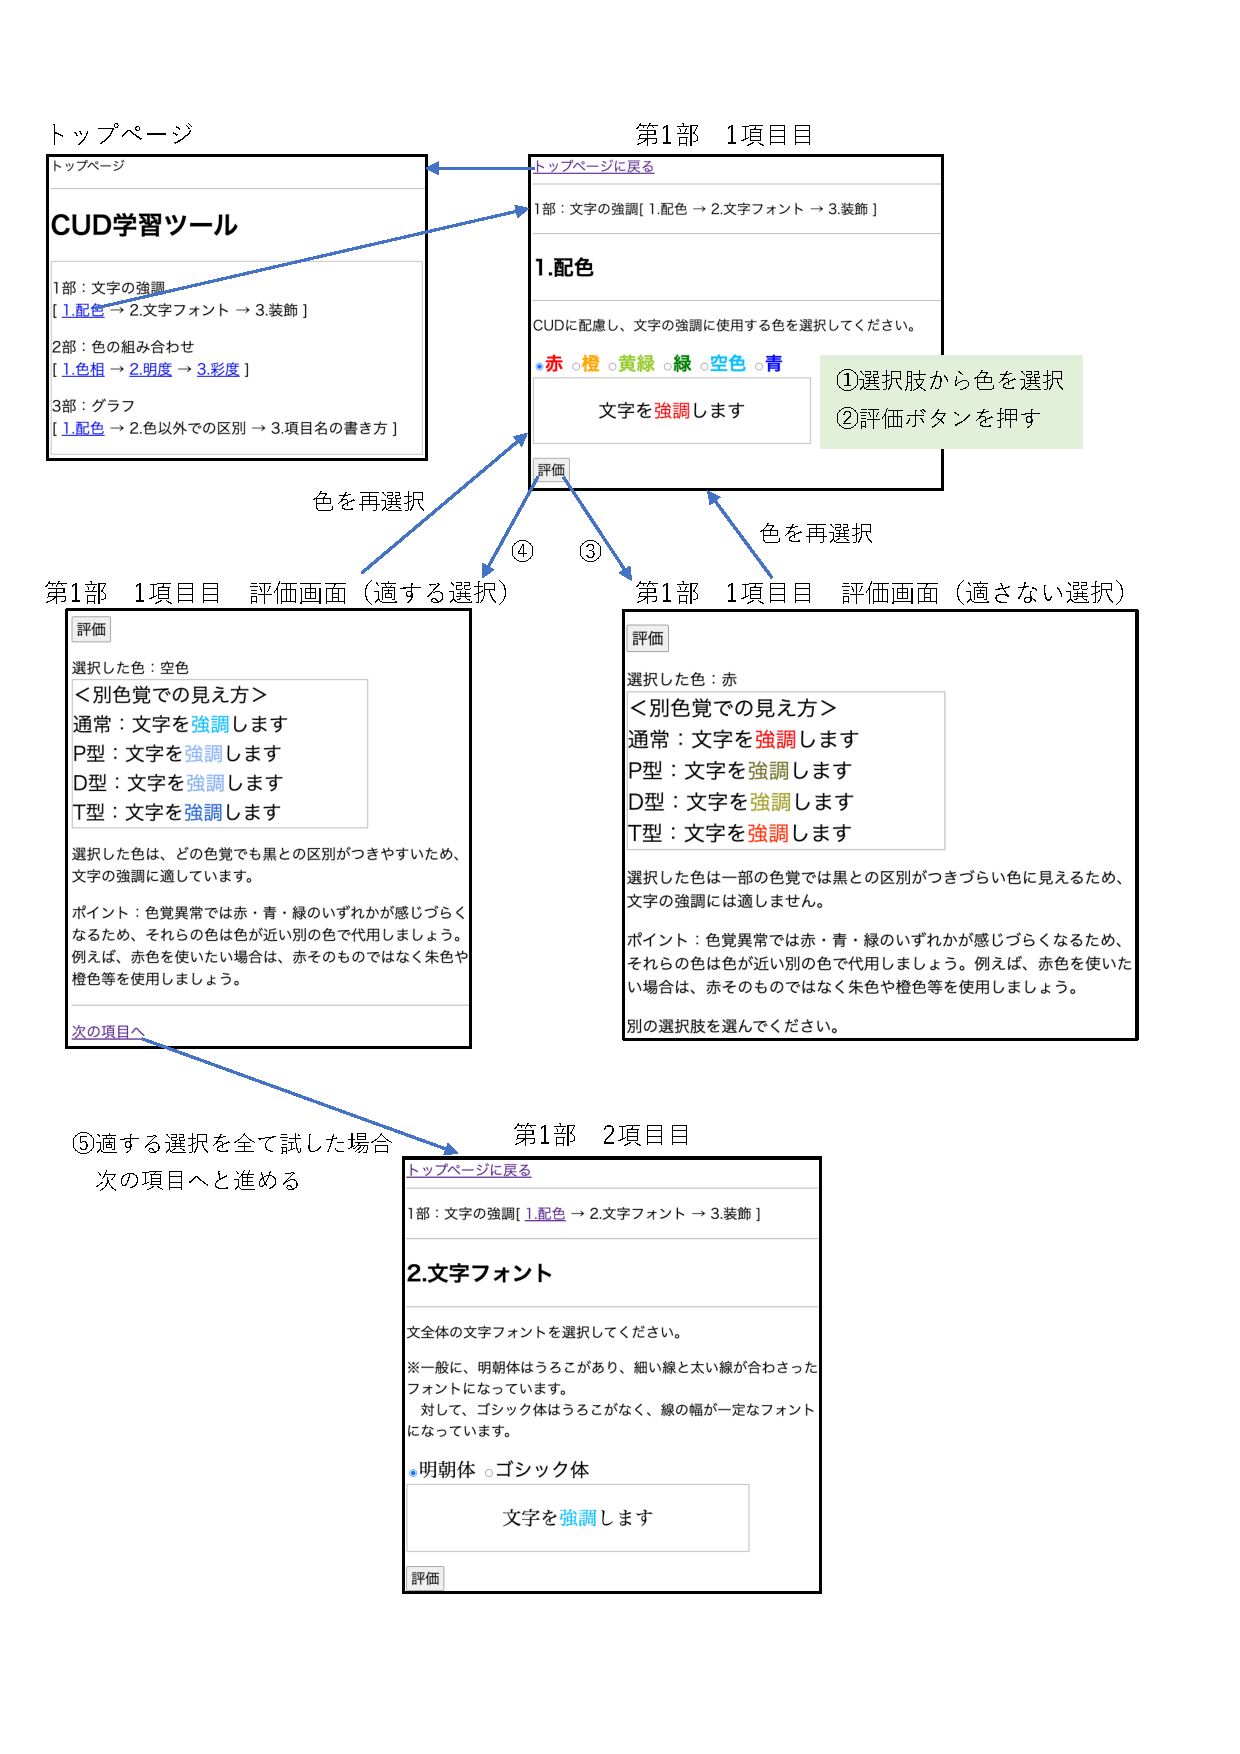
\includegraphics[clip,height=200mm]{images/map.pdf}
\end{center}
 \caption{サイトマップ}
 \label{fig:map}
\end{figure}

\clearpage

\subsection{学習ツールの構成}
本学習ツールは3部構成となっている.

\subsubsection{第1部 文字の強調}
1部では文字の強調を行う際の工夫について学習する.
項目として,配色,フォント,装飾の順に学習する.
図\ref{fig:gamen_1bu}は配色の学習画面である.

配色では,強調に使用する色を選択する.
選択肢は,赤,橙,黄緑,緑,空色,青の6種類である.
色覚異常は赤,青,緑のいずれかが感じづらくなるため,それらは黒との区別がつきづらい色に見える場合がある.
それらの色を選択した場合は文字の強調には適さないという評価とした.

フォントでは,選択肢から文全体のフォントを選択する.
選択肢は明朝体とゴシック体の2種類である.
明朝体には游明朝体やヒラギノ明朝等,複数の明朝体フォントが存在する.
これは,ゴシック体も同様である.
そのため,一概にどちらかが適さないフォントであると断定することは難しい.
一般に,明朝体はうろこがあり,細い線と太い線が合わさったフォントとなっている.
対して,ゴシック体はうろこがなく,線の幅が一定なフォントになっている.
そこでこの学習ツールでは,これらの特徴からCUDの観点で適しているか判断した.
線の一部が細くなっているフォントは色面積が小さくなり,色による判別がつきづらくなるため,色による文字の強調を行う際には適さないという評価とした.

装飾では,選択肢から選択することで,強調する文字を変化させる.
選択肢として,「アンダーラインを引く」と「太字にする」がある.
これらを選択することで,強調する文字を変化させる.
この項目では,色以外で強調を伝える方法を理解させることを目的としているため,これらの選択肢を選択して試した場合に,次の項目に進めるようにした.

\begin{figure}[h]
\begin{center}
 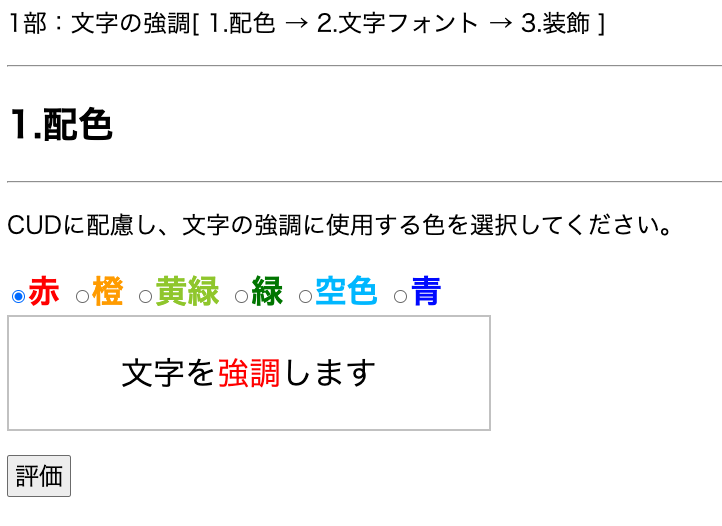
\includegraphics[clip,width=122mm,height=84mm]{images/gamen_1bu.png}
\end{center}
 \caption{1部の学習画面例}
 \label{fig:gamen_1bu}
\end{figure}

\clearpage
\subsubsection{第2部 色の組み合わせ}
2部では,色を組み合わせる際の工夫について学習する.
項目として,色相,明度,彩度の順に学習する.
図\ref{fig:gamen_2bu}は色相での学習画面である.
2部では,全ての項目で,指定された背景色に対する文字の色を選択するという学習の流れとなっており,選択肢が項目によって異なっている.
それぞれ扱っている色のうち1色が背景色となっており,それ以外が選択肢となっている.
背景色は「背景色を変更する」から変更することができる.

色相では,赤,橙,黄色,黄緑,緑,空色,青,紫の8種類を扱っている.
色相とは,赤,緑,青等の色味の種類のことである.
色相で別となっている2つの色の区別がつきづらい場合がある色覚が存在するため,別色覚での見え方を確認した際に,区別がつきづらい配色となる場合は適さないという評価とした.

明度では,明るめの橙,暗めの橙,明るめの緑,暗めの緑の4種類を扱っている.
明度とは,色の明るさのことである.
明度が高いほど白に近づき,低いほど黒に近くなる,
2色を組み合わせる場合は,明度に差をつけることで色覚によらず区別しやすい配色となるため,背景色と同じ明度の色を選択した場合は適さないという評価とした.

彩度では,赤,ピンク,青,水色の4種類を扱っている.
彩度とは,色の鮮やかさのことである.
彩度が高いほど明瞭な原色に近づき,低いほど白や黒等の無彩色に近づく.
彩度が低い色同士で組み合わせると,色による区別がつきづらい場合があるため,それらを組み合わせた場合は適さないという評価とした.

\begin{figure}[h]
\begin{center}
 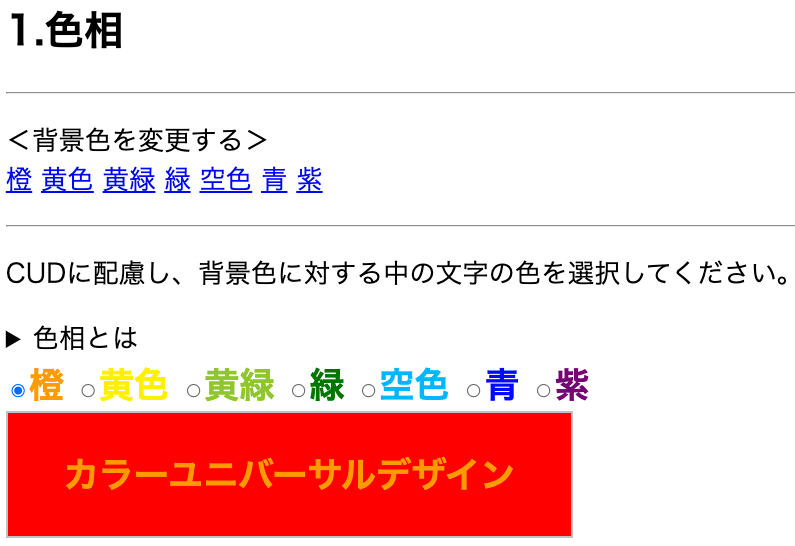
\includegraphics[clip,width=122mm,height=84mm]{images/gamen_2bu.png}
\end{center}
 \caption{2部の学習画面例}
 \label{fig:gamen_2bu}
\end{figure}


\clearpage
\subsubsection{第3部 グラフの作成}
3部では,グラフを作成する際の工夫について学習する.
この学習ツールでは,折れ線グラフを扱った.
項目として,線の色,色以外での区別,項目名の書き方の順に学習する.
図\ref{fig:gamen_3bu}は線の色での学習画面である.
線の色では,グラフに存在する3本の線の配色を選択する.
色の選択肢や配色に対する評価は,2部の1項目目である色相と同じである.

色以外での区別では,線の種類とマーカーの図形を選択する.
線の種類は,実線に加え間隔の異なる破線2種類の合計3種類を扱っている.
マーカーの図形は丸,三角,四角の3種類を扱っている.
線ごとに別々の組み合わせを用いることで,色に頼らず線の区別がつくようになる.
この学習ツールでは線の種類,マーカーの種類がそれぞれ3種類となっているため,それぞれで一つずつ選択していなかった場合は適さないという評価とした.

項目名の書き方では,項目名の表示方法を選択する.
選択肢は,「別枠にまとめる」と「線の近くに表示する」の2種類である.
項目名は,別枠にまとめて表示するのではなく,それぞれの線の近くに表示することで,色に頼らなくとも項目名と線の対応が伝わるようになる.
そのため「別枠にまとめる」を選択した場合は適さないという評価とした.

\begin{figure}[h]
\begin{center}
 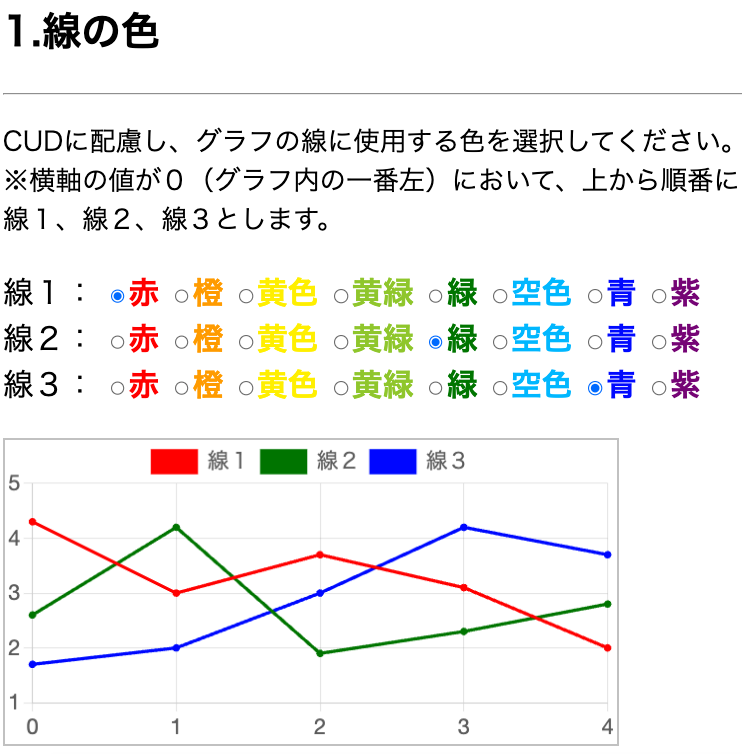
\includegraphics[clip,width=93mm,height=94mm]{images/gamen_3bu.png}
\end{center}
 \caption{3部の学習画面例}
 \label{fig:gamen_3bu}
\end{figure}

\clearpage

%5章
\section{実装方法}

\subsection{概要}
本学習ツールは,学習者がWebブラウザを使用して学習する.

図\ref{fig:sa-ba}は開発したシステムの構成を表している.
本学習ツールでは,クライアントサイドでの要求に対し,サーバサイドで処理を行い,結果を返している.

例として,学習者の選択した内容に対する評価を行う際は,学習者が選択した内容をサーバサイドに送っている.
そして,サーバサイドにあるデータベース(DB)の情報から学習者の選択に対する評価等の情報を取り出し,クライアントサイドに返すことで,学習者側のブラウザに評価等を表示させる.

このように,本学習ツールでは,学習者の選択に対してサーバサイドで処理を行う.

\begin{figure}[h]
\begin{center}
 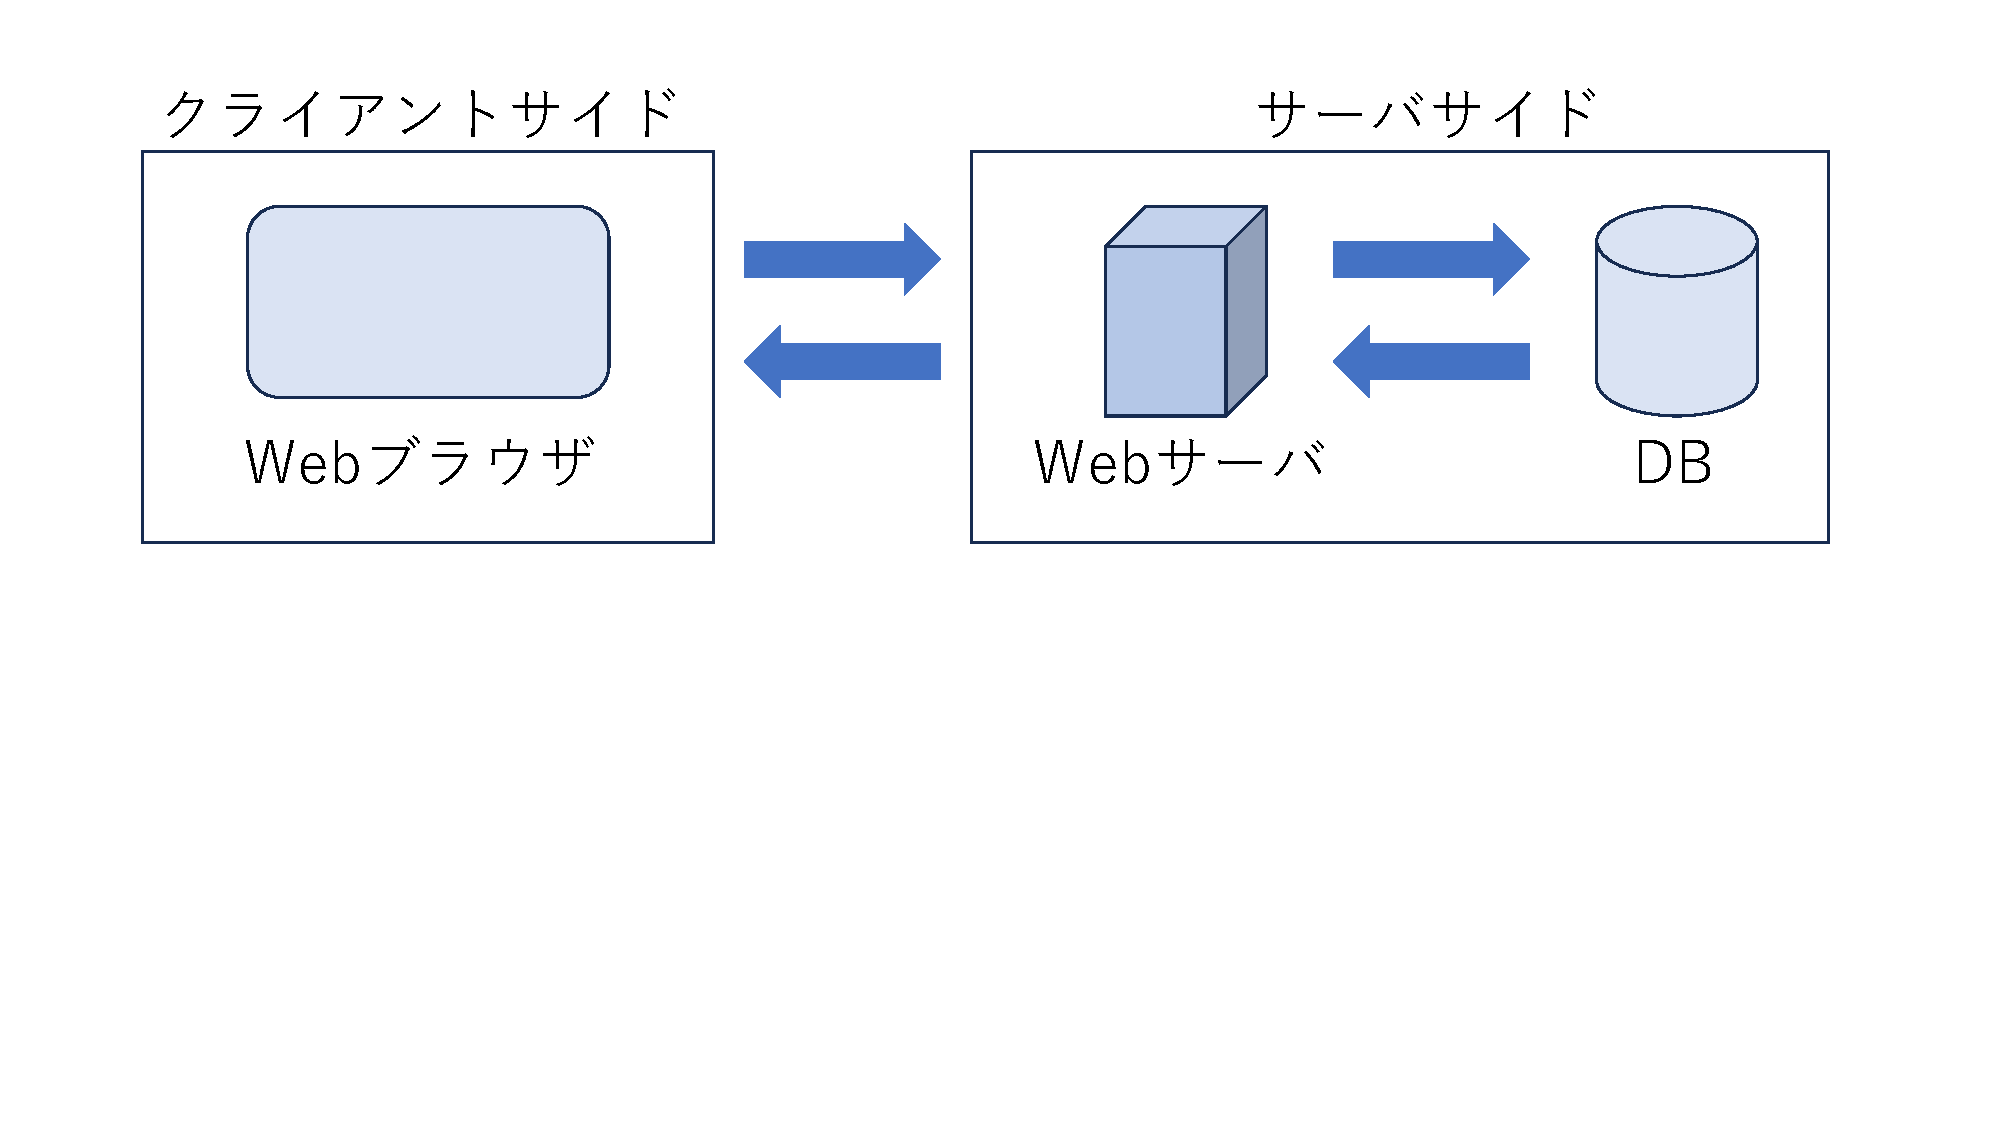
\includegraphics[clip,width=160mm,height=44mm]{images/sa-ba.pdf}
\end{center}
 \caption{開発したシステムの構成}
 \label{fig:sa-ba}
\end{figure}


\subsection{サーバサイド}
\subsubsection{処理内容}
サーバサイドでは,クライアントサイドから送られた情報をもとに,学習者が選択した内容によって表示する評価等を変更する処理を行い,クライアントサイドに結果を返す処理を行う.

\subsubsection{使用している言語}
本学習ツールの開発には,Node.jsのフレームワークの一つであるExpress.jsを利用した.

Node.jsは,サーバーサイドのJavaScript実行環境の一つである.
Node.jsは大量なアクセスに強くリアルタイムの処理に適していること等から,Webアプリケーションの開発等によく使われる.
サーバサイドで学習者の選択によって評価等の表示項目を変更する処理を行うために,サーバーサイドの実行環境であるNode.jsを使用して開発した.

Express.jsはNode.jsのフレームワークの一つである.
Express.jsを利用することで,Node.jsを使用してWebアプリケーションを作成するために必要な機能を容易に実装することができる.
Node.jsを使用した開発を容易にすることを目的として,Express.jsを利用した.

\subsection{DB}
DBには,項目ごとの選択肢や学習者の選択に対する評価に必要な情報等を持たせている.

\subsubsection{DBの設計}
開発したシステムのDBの設計を表\ref{tab:table}に示す.
DBには,textテーブル,colorテーブル,tcテーブル,fontテーブル,evaテーブルの5つのテーブルがある.

\begin{table}[h]
    \caption{テーブル一覧}
   \label{tab:table}
    \centering
    \begin{tabular}{|l||l|l|l|}
        \hline
        テーブル名 & 内容  \\ \hline
        \hline
        text & 項目ごとに表示する文章 \\ \hline
        color & 選択肢となる色の情報 \\ \hline
        tc & 項目と選択肢の対応関係 \\ \hline
        font & 選択肢となるフォントの情報 \\ \hline
        eva & 2色を組み合わせた際の評価 \\ \hline
    \end{tabular}
\end{table}

\subsubsection{DBの詳細}

表\ref{tab:text}はtextテーブルの構成である.
textテーブルには,項目ごとに表示する文章等の情報を格納している.
このテーブルから,評価として表示する文章等を取り出して,学習者に提示している.
idは項目の番号,itemは項目名,queは学習者への指示,goodは学習者の選択が適していた場合の評価,badは適していなかった場合の評価,advはCUDに配慮するためのアドバイスを文章として格納している.

\begin{table}[h]
    \caption{textテーブル}
   \label{tab:text}
    \centering
    \begin{tabular}{|l||l|l|l|}
        \hline
        カラム名 & 内容  \\ \hline
        \hline
        id & 項目番号 \\ \hline
        item & 項目名 \\ \hline
        que & 指示文 \\ \hline
        good & 適した場合の評価 \\ \hline
        bad & 適していない場合の評価 \\ \hline
        adv & アドバイス \\ \hline         
    \end{tabular}
\end{table}

\clearpage
表\ref{tab:color}はcolorテーブルの構成である.
このテーブルには選択肢となる色の情報を格納している.
別色覚での見え方を再現したカラーコード等が入っており,これらのデータを利用して学習者の選択に対して別色覚での見え方を表示している.
idは番号,nameは色の名前,ccodeは色のカラーコード,pcode,dcode,scodeは別色覚での見え方を再現したカラーコードを色覚ごとに格納している.

\begin{table}[h]
    \caption{colorテーブル}
   \label{tab:color}
    \centering
    \begin{tabular}{|l||l|l|l|}
        \hline
        カラム名 & 内容  \\ \hline
        \hline
        id & 番号 \\ \hline
        name & 名前 \\ \hline
        ccode & カラーコード(通常の色覚) \\ \hline
        pcode & カラーコード(P型色覚) \\ \hline
        dcode & カラーコード(D型色覚) \\ \hline
        scode & カラーコード(T型色覚) \\ \hline         
    \end{tabular}
\end{table}

表\ref{tab:tc}はtcテーブルの構成である.
このテーブルは,textテーブルとcolorテーブルの中間テーブルである.
項目ごとに選択肢となる色が異なるため,項目と選択肢の対応関係を格納している.
t-idはtextテーブルのid,c-idはcolorテーブルのidを表す.

\begin{table}[h]
    \caption{tcテーブル}
   \label{tab:tc}
    \centering
    \begin{tabular}{|l||l|l|l|}
        \hline
        カラム名 & 内容  \\ \hline
        \hline
        t-id & 項目番号 \\ \hline
        c-id & 色番号 \\ \hline   
    \end{tabular}
\end{table}

%\clearpage
表\ref{tab:font}はfontテーブルの構成である.
このテーブルには,文字の強調について学ぶ際の選択肢となるフォントの情報を格納している.
idは番号,faceはCSSでフォントを指定する際の値,nameはフォントの名前,gbはCUDに配慮したフォントであるかを0か1で格納している.

\begin{table}[h]
    \caption{fontテーブル}
   \label{tab:font}
    \centering
    \begin{tabular}{|l||l|l|l|}
        \hline
        カラム名 & 内容  \\ \hline
        \hline
        id & 番号 \\ \hline
        face & 値 \\ \hline
        name & 名前 \\ \hline
        gb & 評価 \\ \hline
    \end{tabular}
\end{table}

\clearpage
表\ref{tab:eva}はevaテーブルの構成である.
このテーブルには,2色のカラーコードと組み合わせた際の評価となる情報を格納している.
2色を組み合わせた際に色覚異常の見え方でも区別がつきやすい組み合わせかどうかこのテーブルの情報をもとに判断している.
cola,colbはそれぞれ別のカラーコード,gbはその2色の組み合わせがCUDに配慮されているかを0か1で格納している.

\begin{table}[h]
    \caption{evaテーブル}
   \label{tab:eva}
    \centering
    \begin{tabular}{|l||l|l|l|}
        \hline
        カラム名 & 内容  \\ \hline
        \hline
        cola & カラーコード1 \\ \hline
        colb & カラーコード2 \\ \hline
        gb & 評価 \\ \hline
    \end{tabular}
\end{table}




\subsubsection{使用したDB}
DBにはSQLiteを使用している.
SQLiteはアプリケーションに組み込むことで利用する簡易的なDBである.
主要なデータベースに比べて大規模なWebアプリには不向きな反面,セットアップが容易であるため,本学習ツールではSQLiteを利用した開発を行った.







\clearpage

%6章
\section{検証}
この章では,開発した学習ツールを用いて行った検証について説明する.

\subsection{実施内容}
開発した学習ツールを用いて,学生10名を対象に検証した.
対象者には,東京都が作成したCUDのガイドラインを参考に色覚異常とCUDについて事前に説明した\cite{tokyo}.
そして,対象者には学習ツールを利用した後に,Microsoft PowerPointを用いてスライドを作成してもらった.
そのスライドをCUDに配慮されているか項目別に評価した.

\subsection{評価項目}
評価項目は,適切なフォント,色の組み合わせ,強調目的の色,ハッチング,装飾の5項目である.
これは先行研究での評価項目に,装飾に関する項目を加えた.
配色に関する項目については,医学及びメディアデザイン学の博士号を持つ作者が開発した色のシミュレータを用い,通常の色覚に加え,P型色覚,D型色覚,T型色覚での見え方を確認し評価した\cite{simulator}.

「適切なフォント」では,使用しているフォントがCUDに配慮されているか評価した.
線の一部が細くなっているフォントは色面積が小さくなり,色による判別がつきづらくなるため,色による文字の強調を行う際には適さないフォントである.
そのため,線の幅が一定なフォントが使用されているかという観点で評価した.

「色の組み合わせ」では,2色を組み合わせて使用する場合に,どの色覚であっても区別がつきやすい配色となっているか評価した.

「強調目的の色」では,文字の一部の色を別の色にすることで強調する場合に,どの色覚でも強調していることが伝わりやすい配色となっているか評価した.
通常の色覚では黒と明確に区別できる色でも,別の色覚では黒と区別がつきづらい色に見える場合がある.
複数の色覚での見え方を確認し,どの色覚でも明確に区別がつき,強調が伝わる配色となっているか評価した.

「ハッチング」では,折れ線グラフを作成する際に,それぞれの線を色以外の情報で区別できるようになっているか評価した.
折れ線グラフを作成する際は,実線と破線を組み合わせ,マーカーの図形を線ごとに別の種類にすることで,色に頼らずに線を区別できるため,色覚によらず伝わりやすいグラフとなる.
これらの工夫が取り入れられているか評価した.

「装飾」では,色以外で文字の強調が伝わる資料となっているか評価した.
文字を強調する際は,配色に加え,アンダーラインを引くことや,強調する文字を太くする等を行うことで,色以外の情報で文字の強調を伝えることができる.
これらの工夫が取り入れられているか評価した.

\clearpage

%7章
\section{結果}
項目ごとに,CUDに配慮した工夫が取り入れられていた資料の割合を図\ref{fig:result}に示す.

配色に関する項目について,
強調目的の色でCUDに配慮されていた資料は90%であり,先行研究に比べて10ポイント増加している.
色の組み合わせでは,全ての資料がCUDに配慮した配色となっていた.

色以外の工夫に関する項目について,
適切なフォントでは,全ての資料がCUDに配慮したフォントとなっていた.
また,ハッチングでCUDに配慮されていた資料は90%であった.
一方,新たに評価項目として加えた装飾でCUDに配慮されていた資料は70%であった.

\begin{figure}[h]
\begin{center}
 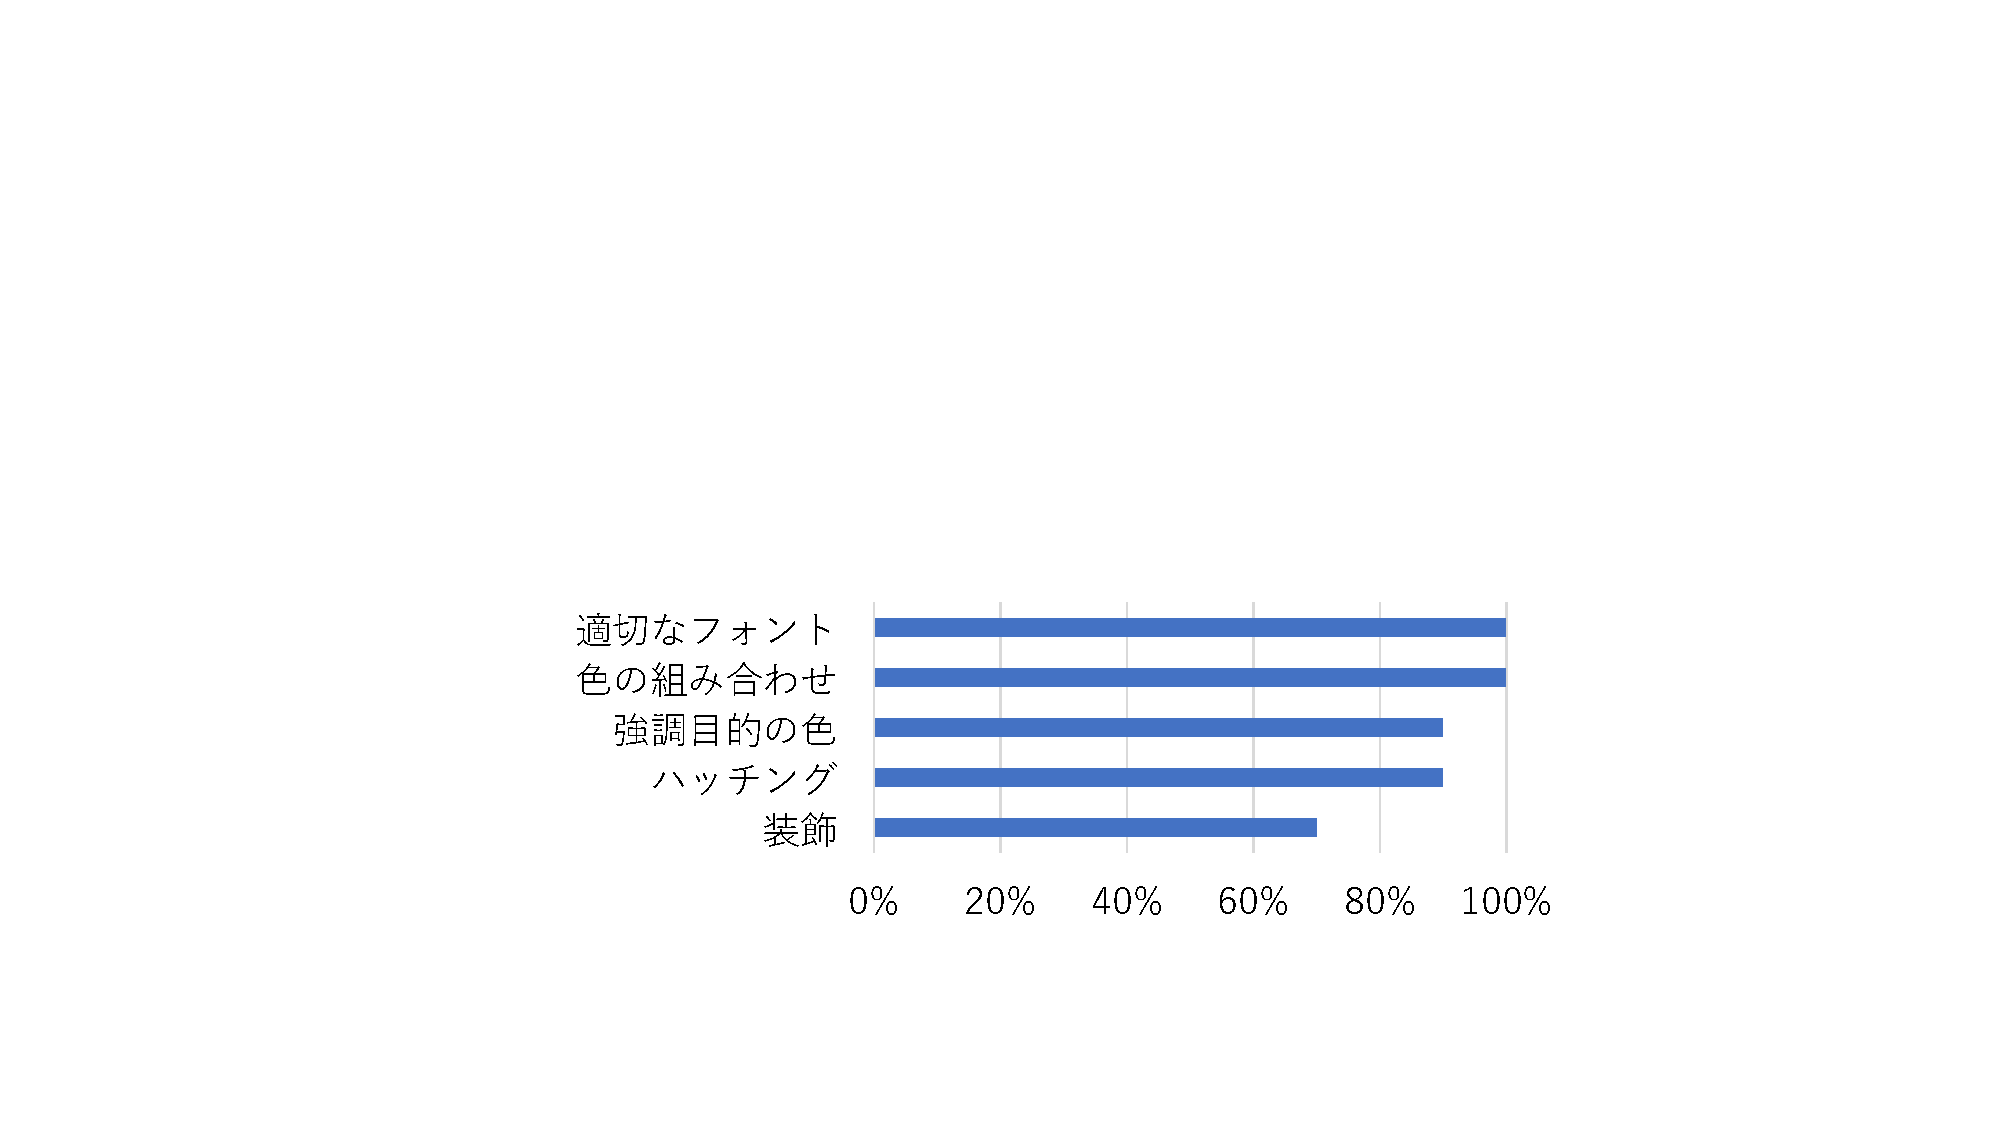
\includegraphics[clip,width=110mm,height=38mm]{images/result.pdf}
\end{center}
 \caption{CUD評価結果}
 \label{fig:result}
\end{figure}

%\clearpage

%8章
\section{考察}
配色に関する項目で,先行研究に比べてCUDに配慮した資料が増加している.
開発した学習ツールを利用することで,CUDに配慮した資料を作成できるという結果が得られた.
そのため,学習者がCUDに配慮した工夫を項目ごとに実践することで,CUDに配慮した資料を作成できると考えられる.
また,配色に関する項目でCUDに配慮した資料が増加した要因として,本学習ツールで別色覚での見え方や評価を即座に確認できるようになったことで,様々な配色を試すことが容易であったことが考えられる.

一方,評価項目の一つである装飾の観点では,CUDに配慮された資料は70%であった.
本学習ツールでは,配色に関する項目の後に装飾を学習する.
複数の色覚で区別がつきやすい配色を行った後に装飾に関する工夫を実践する流れであることや,配色と異なり複数回試すことがない項目であることから,装飾の重要性が伝わりにくくなっていたと考えられる.
これらから,学習の流れや表示項目を改善することが望ましい.
\clearpage

%9章
\section{結言}
遺伝子の異常により通常と色の見え方が異なる色覚を持つ色覚異常者は,男性で5%,女性で0.2%存在する.
色覚の多様性に配慮し,より多くの人に伝わりやすいデザインとしてカラーユニバーサルデザイン(CUD)がある.

学生や社会人になると,ゼミや業務等で資料を作成する機会が増加する.
そのため,CUDの講習では資料作成を実践し評価する機会が設けられている.
しかし,講習を受けた学生の20%がCUDに配慮していない資料を作成した.

本研究では,CUDに配慮した工夫を一つ一つ実践する機会が必要だと考え,これらを行える学習ツールを開発した.
開発した学習ツールを学習者が利用した結果,配色に関する項目で,先行研究に比べてCUDに配慮した資料が増加した.
このことから,開発した学習ツールを利用することで,CUDに配慮した資料を作成できるという結果が得られた.
一方,評価項目の一つである装飾の観点でCUDに配慮された資料は70%であり,他項目に比べて工夫が行われていないため,学習の流れや表示項目等の改善が望まれる.
\clearpage

%謝辞
\section*{謝辞}
\addcontentsline{toc}{section}{謝辞}
本論文の執筆にあたりご指導くださった須田先生に感謝申し上げます.
また,研究室のメンバーには多くの手助けを頂きました.
 本当にありがとうございました.
\clearpage

%参考文献
\begin{thebibliography}{99}

\bibitem{okabe}岡部正隆・伊藤啓・橋本知子: ``ユニバーサルデザインにおける色覚バリアフリーへの提言'', \url{https://www.nig.ac.jp/color/handout1.pdf}, 2024/1/9参照

\bibitem{sugamiya} 菅宮恵子: ``色覚異常を考慮した教材資料作成実習の実践報告とその評価'', 教職・学芸員課程研究,2号(2020),p.14-23, 2024/1/9参照

\bibitem{tokyo} 東京都福祉保健局生活福祉部地域福祉推進課: ``東京都カラーユニバーサルデザインガイドライン'', \url{https://www.fukushi.metro.tokyo.lg.jp/kiban/machizukuri/kanren/color.files/colorudguideline.pdf},2024/1/9参照

\bibitem{osaka} 府民文化部府政情報室広報広聴課: ``色覚障がいのある人に配慮した色使いのガイドライン'', \url{https://www.pref.osaka.lg.jp/koho/shikikaku/guide1.htmlf},2024/1/9参照

\bibitem{jcolor} 一般社団法人日本カラーコーディネーター協会: ``大阪医療福祉専門学校様 特別授業「CUD」のご報告'', \url{https://www.j-color.or.jp/2023/03/15/blog-entry-884/},2024/1/9参照

\bibitem{simulator}浅田一憲: ``色のシミュレータ'', \url{https://asada.website/cvsimulator/j/index.html},2024/1/9参照




\end{thebibliography}

\clearpage

%付録
\appendix
\section{作成したプログラム}

\subsection{app.js}
\label{app.js}
\listinginput{1}{./input/app.js}
\newpage

\subsection{layout-1a.ejs}
\label{layout-1a.ejs}
\listinginput{1}{./input/layout-1a.ejs}
\newpage

\subsection{func.js}
\label{func.js}
\listinginput{1}{./input/func.js}
\newpage
\clearpage

\end{document}